\chapter{Surface realization --- evolving programs using AlphaEvolve}
\label{chap:surface-realization}

\section{Method Overview}
\label{sec:surface-method-overview}

The previous chapter considered the problem of meaning representation construction. Complex
structured data was converted into semantic triples so that the information
could be expressed in a compact, standardized, and machine-interpretable form.
The problem considered in this
chapter is the second stage of the data-to-text conversion: given the
information contained in a set of triples, how should it be written in natural
language?

This stage is called \emph{surface realization}. Let
$T = \{(s_i,p_i,o_i)\}_{i=1}^{n}$ denote a set of subject--predicate--object
triples and let $y$ denote a natural-language text. A surface realizer is a
mapping
\begin{equation}
    G : T \longrightarrow y,
\end{equation}
which must express the facts in $T$ fluently and coherently. The mapping is not
limited to replacing predicates with fixed phrases. It can require entity
ordering, aggregation of related facts, selection of referring expressions,
realization of numerical values, and the choice of a suitable sentence
structure. The generated text should preserve the information in the triples
while avoiding unsupported statements and unnecessary repetition.

An LLM can perform this mapping directly for every input through a zero-shot or
few-shot prompt. That approach can produce fluent text, but the realization decision is
then made anew for each input. This thesis instead uses the LLM to propose changes to a
Python surface-realization program. The resulting program is a reusable artifact:
after an evolutionary run, it can be inspected and executed on previously unseen
triple sets without another LLM call.

This idea is directly motivated by the work of Lango and Dusek~\cite{lango-dusek-2025-llm},
who describe a neurosymbolic framework in which LLM agents implement an NLG
system from scratch. The generated code provides a transparent
representation of the realization process and can generate text using ordinary
CPU execution. The work demonstrates that LLMs can be used to build an NLG
system rather than only to act as the NLG system at inference time.

The present work shares the goal of an inspectable generator, but
obtains it differently. Here, Google's AlphaEvolve idea is
used instead~\cite{novikov2025alphaevolve}: rather than assigning several agents the task of
designing and refining a program, it starts from a working baseline and searches
over LLM-proposed program mutations. Each candidate is executed and selected
using a task-specific objective. Unlike the reference-free construction setting
of Lango and Du\v{s}ek, this search uses reference
lexicalizations, to evaluate candidate programs.
The method is therefore an LLM-guided evolutionary algorithm 
in which an LLM mutates a program to complete a general
software-engineering task. Its loop is as follows:
\begin{enumerate}
  \item select a previously evaluated parent program;
  \item ask a selected LLM to propose a mutation of that program;
  \item execute the mutated program on evaluation inputs;
  \item calculate a scalar selection score or a diagnostic feedback; and
  \item register the candidate so that it can influence later selection.
\end{enumerate}
The remainder of the chapter introduces the related programming paradigms,
defines AlphaEvolve's evolutionary formulation, and then describes the
OpenEvolve implementation and its evaluation modes.

\section{Program construction and coding agents}
\label{sec:modern-programming}

Program synthesis searches for a program consistent with a formal specification
or a set of input--output examples. Code completion, in contrast, predicts a
local continuation of an existing source file. Neither description by itself
implies an iterative development process. \emph{Agentic programming} denotes a
different setting in which an LLM-based system maintains a control loop: it
observes a workspace, invokes tools, interprets their results, and chooses later
actions while pursuing a software-development task
\cite{wang2025agenticprogramming}.

The distinction matters here because the later described AlphaEvolve uses some ideas common in
coding-agent systems---a language model, source code, execution feedback, and
persistent state---without requiring a general tool-using agent. It has a
restricted interface: the LLM proposes a program mutation and an evaluator
returns its result. This restricted loop makes candidate comparison explicit and
repeatable, which is useful when the desired artifact is a compact surface
realizer rather than a complete software project.

Coding agents nevertheless motivate the use of execution feedback. Generated
source can contain invalid assumptions or fail a test. 
The relevant question for this chapter is consequently not
whether an LLM can describe a realization strategy, but whether the resulting
program improves an observable realization objective. AlphaEvolve provides the
selection mechanism for this question.

\section{AlphaEvolve}
\label{sec:alphaevolve}

\subsection{Evolutionary formulation}

AlphaEvolve is an LLM-guided evolutionary coding system for scientific and
algorithmic problems whose candidate solutions can be represented as programs
and evaluated automatically~\cite{novikov2025alphaevolve}. Let $\mathcal{P}$
denote programs satisfying a task interface and let
\begin{equation}
    h : \mathcal{P} \longrightarrow \mathbb{R}^{m}
\end{equation}
be an evaluator that returns one or more metrics. A designated scalar derived
from these metrics is the fitness used for selection. Beginning with a runnable
baseline $p_0$, the system repeatedly selects a parent $p$, obtains an
LLM-proposed mutation $p'$, evaluates $h(p')$, and stores the result. The stored
programs then form the pool from which later parents are sampled.

The LLM generation is stochastic,
but a generated program is an ordinary deterministic source artifact until it
is changed again. The LLM replaces a hand-designed mutation operator by proposing
source-level modifications that may express algorithmic ideas. Selection is
still based on the evaluator, rather than on the persuasiveness of the LLM's
explanation.

\subsection{Architecture}

The description of AlphaEvolve separates the process of creating a program into the
following cooperating components~\cite{novikov2025alphaevolve}:

\begin{enumerate}
  \item The \emph{task specification} supplies the initial program, the
  evaluator, optional configuration, and any fixed domain knowledge.
  \item The \emph{prompt sampler} selects previously evaluated programs and
  assembles the context shown to the language model.
  \item The \emph{LLM ensemble} asks a selected LLM to propose a mutation of that program. A routing or
  sampling policy selects one model for a mutation request; that model independently
  returns a candidate patch. Faster models can be sampled more often to explore
  more candidates, while a more capable model can be selected for less frequent changes
  \item The \emph{mutation layer} parses the model response and applies the
  proposed changes to the current source code. For large programs, targeted
  diff blocks avoid sending or rewriting unrelated code.
  \item The \emph{evaluators} execute the candidate and return its metrics.
  Evaluation can include cascades, parallel test cases, multiple objectives,
  and additional LLM-generated feedback.
  \item The \emph{program database} stores candidates, metrics and controls
  the balance between exploiting high-scoring programs and exploring different
  program structures.
  \item The \emph{distributed controller} coordinates LLM requests and
  evaluations asynchronously so that slow evaluations do not prevent other
  candidates from being processed.
\end{enumerate}

The interaction between these components is deliberately cyclic. The program scores, code, and observed failures become part of the context used for subsequent mutations.
The database consequently acts as an external memory for the LLM-guided evolutionary algorithm
agent.~\cite{novikov2025alphaevolve}.
The following sections describe the components in more detail.

\begin{figure}[ht]
    \centering
    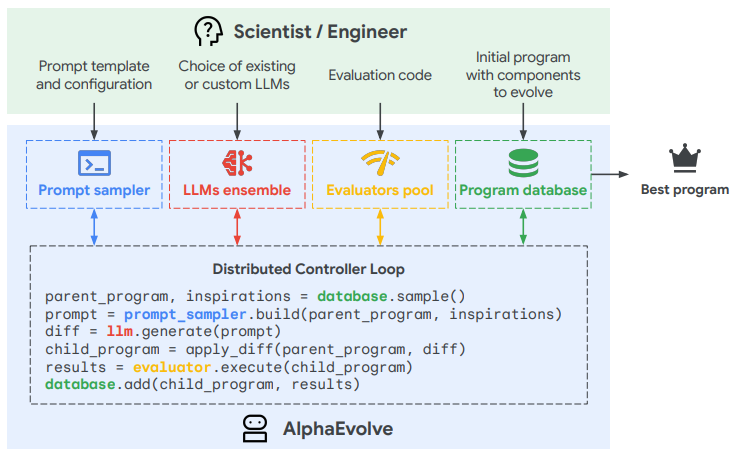
\includegraphics[width=\textwidth]{figures/alpha-evolve.png}
    \caption{The AlphaEvolve program-evolution process, adapted from
    Novikov et al.~\cite{novikov2025alphaevolve}.}
    \label{fig:alpha-evolve}
\end{figure}

\subsection{Task specification and program representation}

An AlphaEvolve task has three essential inputs. First, an initial program must
be complete enough to run, even if its implementation is deliberately simple
(the complete initial program is reproduced in Appendix~\ref{app:initial-program}).
Second, the part of the source code that may be changed is marked with
\texttt{\# EVOLVE-BLOCK-START} and \texttt{\# EVOLVE-BLOCK-END}. The remaining
code forms a fixed skeleton that defines imports, data types, and the public
interface. Third, an evaluator function must be provided. The evaluator
receives the generated program, executes it on the task-specific inputs, and
returns a dictionary of scalar metrics.

\subsection{Prompt sampling and creative generation}

AlphaEvolve prompts contain more than the current program. Depending on the
configuration, the context can contain high-scoring programs, structurally
diverse programs, previous attempts, evaluator outputs, artifacts, explicit
human-written instructions, and relevant examples or literature. The complete
experiment-specific prompt composition is shown in Appendix~\ref{app:prompts-evolution}.
This context allows an LLM to compare alternatives rather than repeatedly
proposing a mutation without knowing what has already been tried.

The LLM is asked to make a concrete source-level change. For a diff-based
mutation, the expected response is a sequence of blocks of the form
\begin{quote}
\texttt{<<<<<<< SEARCH}\\
\texttt{original code}\\
\texttt{=======}\\
\texttt{replacement code}\\
\texttt{>>>>>>> REPLACE}
\end{quote}
The search part identifies the source segment to be replaced, and the replace
part contains the candidate implementation. The complete mutation template is
provided in Appendix~\ref{app:prompt-evolution-user}. A complete rewrite can be used for
short programs or when a targeted change is not appropriate. In both cases,
the model is instructed to preserve the public interface and to optimize the
metrics defined by the evaluator.

AlphaEvolve uses an ensemble rather than relying on only one generation model.
In the original system, a faster model increases the number of explored ideas,
while a more capable model can supply less frequent but more substantial
changes~\cite{novikov2025alphaevolve}. The ensemble is not an ensemble in the
sense of averaging source code. A single model response is selected for each
mutation, after which the resulting program is evaluated independently.

\subsection{Evaluation, evolutionary storage, and distributed execution}

AlphaEvolve supports several mechanisms for making the evaluation stage both
useful and affordable. An evaluation cascade can apply inexpensive tests first
and run expensive tests only for candidates that pass earlier thresholds.
Parallel test cases can be distributed across workers. Multiple
metrics can be returned simultaneously, both because they may represent genuine
objectives and because programs that perform well under different metrics can
provide more varied context for future mutations. Optional LLM feedback can be
used for properties that are difficult to express in a conventional evaluator,
such as readability or simplicity.

The system is implemented as an asynchronous pipeline. LLM generation and
evaluation are started whenever their required inputs are available, and the
controller waits only at dependencies between stages. This maximizes the
number of candidates evaluated within a fixed computation budget instead of
minimizing the latency of an individual candidate.

\subsection{Scope and limitations of AlphaEvolve}

The unique feature of AlphaEvolve is the combination of open-ended LLM
mutations with machine-gradeable selection. It is not a general replacement
for a software engineer, and it cannot be applied directly when candidate
quality cannot be measured by an evaluator. Its results depend on the quality,
coverage, and resistance to exploitation of the evaluation function. A weak
metric can reward a program that optimizes the measurement rather than the
intended task. The search can also require substantial computation because
many candidates must be generated and evaluated, and there is no general
guarantee that the best program will be found within a finite budget.

\section{OpenEvolve}
\label{sec:openevolve}

\subsection{Open-source implementation}

OpenEvolve is an open-source implementation of the AlphaEvolve design~\cite{sharma2025openevolve}
and is used as the execution framework for all surface-realization experiments.
The implementation exposes the same basic interface as AlphaEvolve: an initial
program, an evaluator, and a configuration determine an iterative process in
which programs are proposed, scored, and registered for future use.

The main controller loads the
initial source, initializes the LLM ensemble, prompt sampler, evaluator, and
program database.
The initial program is evaluated before the evolutionary workers are started. On a
fresh run it is then inserted into the database as generation zero. This makes
the baseline available to the selection mechanism and ensures that evolution
starts from a measured candidate rather than an unscored source file.

\subsection{Execution architecture used in the thesis}

The local implementation uses parallel workers for
process-based parallelism. Before a worker is submitted, the controller selects
a parent program and inspiration programs, which are selected the same way as the parent
program, and are used as a source of inspiration for the LLM. Then the controller builds the prompt, calls the LLM,
parses the response, and evaluates the resulting source.

Consequently, the logical evolution loop is:

\begin{enumerate}
  \item select a parent and inspirations;
  \item assemble a prompt from the selected context;
  \item generate and parse an LLM mutation;
  \item execute the candidate evaluator;
  \item register the candidate, metrics, and feedback;
  \item repeat until the iteration budget, target score, or stopping rule is
  reached.
\end{enumerate}

The implementation is asynchronous in practice. Several workers can use
snapshots of the program database made close together, and their results can be incorporated in a
different order from the numerical iteration identifiers. This increases
throughput but means that a candidate does not necessarily use the immediately
preceding candidate as its parent.

\subsection{Extensions made for the experiments}

Several changes were made to the OpenEvolve's algorithm. They address
both the search distribution and the failure modes that are common when a
language model is required to emit an exact source-code patch.

\paragraph{Fitness-weighted and island-specific selection.}
The database was extended with roulette-wheel selection. Parent and inspiration
programs can be sampled with probabilities derived from their fitness instead
of being selected uniformly. A small positive lower bound is used in the
fitness weights so that low-scoring programs are not removed from consideration
immediately. LLM configurations can also be assigned to islands, allowing a
population to be associated with a particular model or model mixture. An
optional iteration-based model schedule was added for periodically forcing a
chosen model.

\paragraph{Configurable inspirations.}
The number of inspiration programs that are selected and added to the prompt can be controlled.

\paragraph{More robust SEARCH/REPLACE application.}
The original exact line matching was extended with trailing-whitespace cleanup
and common-indentation handling. A model can therefore return a source block
with a different outer indentation while the replacement is still inserted at
the correct nesting level. If the response has no parsable diff, a corrective prompt asks the
LLM to return the required format. If a syntactically valid diff does not
change the source because its SEARCH block does not match, a second corrective
prompt includes the parent code and asks the LLM to repair the SEARCH section.
The exact repair prompts are given in Appendix~\ref{app:prompt-repair}.

\paragraph{Retention of failed candidates.}
Malformed or unchanged proposals are written to a separate
directory instead of being silently discarded.
Duplicate source code is detected before insertion.
These changes prevent repeated evaluation of identical candidates and preserve
evidence needed to diagnose the behavior of the LLM and the mutation parser.

\paragraph{Explicit zero scores for timeouts.}
The evaluator integration was changed so that timeout and failed-evaluation
paths give a score of 0.

\section{Program database and initial program}
\label{sec:program-database}

\subsection{Program records and persistence}

The program database is implemented in a way to store those principal fields:

\begin{itemize}
  \item a unique identifier and the program source;
  \item the identifier of the parent program, generation number, timestamp, and
  iteration at which the program was found;
  \item a dictionary of evaluation metrics, including the fitness metric;
  \item derived values such as complexity and diversity and metadata such as
  island assignment and a human-readable change summary;
  \item optional prompts and LLM responses associated with its creation;
  \item optional artifacts and embeddings used for feedback and novelty
  checks.
\end{itemize}

The active database is maintained in memory for fast selection.
For each program, feature coordinates are calculated before insertion.

At most one program is retained as the occupant of a feature cell. If a new
program maps to an empty cell, the cell is occupied. If it maps to an occupied
cell, the program with the better fitness is retained as the cell occupant.
The database separately stores a bounded set of elite programs. The absolute
best program is tracked independently so that it is protected from ordinary
population cleanup. When the configured population limit is exceeded, the
lowest-fitness unprotected programs are removed from the active in-memory
population, together with their references in islands and cells. The main limits are configurable.

\subsection{Initial program}

The initial program, reproduced in Appendix~\ref{app:initial-program}, defines a small \texttt{Triple} data class with
\texttt{subject}, \texttt{predicate}, and \texttt{object} fields. Its evolution
block contains the following baseline behavior: \texttt{predict} receives a
list of triples and returns a
generic sentence for the first triple only:
\begin{quote}
\texttt{The \{predicate\} of \{subject\} is \{object\}.}
\end{quote}
This implementation is intentionally minimal. It
is syntactically valid and satisfies the interface, but it ignores additional
triples, treats every predicate identically, and does not model relations
between entities.

The purpose of evolution is not merely to make this baseline longer. The
desired search direction is from a generic fallback sentence towards a
domain-aware surface realizer. Useful changes include mapping predicates to
natural-language templates, grouping triples by subject, identifying a main
entity, ordering attributes, joining related entities, selecting relative
clauses, and maintaining grammatical agreement. These changes are evaluated
by the generated text rather than being prescribed as a fixed hand-written
algorithm, which allows multiple realization strategies to be explored.

\section{Program selection and prompt engineering}
\label{sec:program-selection}

\subsection{Parent and inspiration selection}

Selection is performed before a worker process is launched. For roulette
selection, the parent is selected from the island using a
fitness-weighted softmax distribution. The use of a distribution
rather than always selecting the best program retains a non-zero probability
of returning to less explored solutions.

Inspirations are selected separately from the parent. They are alternative
programs that can provide a design idea without being the source that is
directly modified. With roulette, their probabilities are
also based on fitness, and the parent itself is excluded from the candidate
inspiration set. The selected parent and inspirations are
passed to the worker, which reconstructs their source code from the database.

\subsection{Prompt composition}

The system message used for the surface-realization experiment is reproduced in
Appendix~\ref{app:prompt-evolution-system}. It contains four kinds of fixed
information:

\begin{itemize}
  \item the role of the model as an expert data engineer;
  \item the description of the data to be processed and the required \texttt{predict} function signature;
  \item an example in which several triples are combined into one complex
  sentence;
  \item the list of predicates that may occur, with one example triple for
  each predicate.
\end{itemize}

The user message is assembled for each selected parent. Its complete template
and runtime components are shown in Appendix~\ref{app:prompt-evolution-user}.
Its main parts are:

\begin{itemize}
  \item the current metrics and fitness score;
  \item optional evaluator artifacts, such as low-scoring triples and the
  generated text that caused them (see Appendix~\ref{app:prompt-artifact-message});
  \item the complete current source code;
  \item the mutation task, including the requirement to improve
  the score, preserve the interface, and use the exact
  SEARCH/REPLACE format.
\end{itemize}

Consequently, the code and score of the selected parent are shown directly in
the current-program section. An inspiration is rendered separately with its
own score and source code. A high-scoring program can therefore provide a
strong implementation pattern, while a structurally different inspiration can
suggest a different way of grouping or ordering triples.

\subsection{SEARCH/REPLACE instructions and their extensions}

The mutation prompt asks for a targeted edit rather than a complete rewritten
file. The SEARCH section must identify source text present in the current
program, and the REPLACE section must contain the proposed replacement. The
controller extracts all matching blocks with a regular expression, applies
them line by line, and checks whether the resulting source differs from the
parent. This format makes changes auditable and reduces the risk that the LLM
rewrites fixed parts of the program unintentionally. The full mutation prompt
is given in Appendix~\ref{app:prompt-evolution-user}.

The format is also a significant source of failure. A model can describe a
patch in prose, omit one of the delimiters, copy an outdated version of the
source, or use an indentation that prevents an exact match. These problems
are adressed in two ways. First, trailing whitespace
is normalized and common indentation is removed while matching, after which
the replacement is re-indented at the original location. Second, malformed
responses and unapplied responses are sent to dedicated repair prompts. These
safeguards preserve the replacement text where possible and focus the subsequent
LLM call on producing a matchable SEARCH section; the repair messages are
listed in Appendix~\ref{app:prompt-repair}.

\section{Large Language Model}
\label{sec:large-language-model}

\subsection{Parsing the LLM response}

OpenEvolve uses an OpenAI-compatible client interface, so the same orchestration
code can communicate with hosted models or local servers. The response is
processed in the worker in the following order:

\begin{enumerate}
  \item The response is searched for one or more SEARCH/REPLACE blocks.
  \item Each block is normalized into source lines and applied to the parent
  source.
  \item If at least one block is found but no source line is changed, the
  response is treated as an unapplied mutation rather than as a successful
  no-op.
  \item A new identifier is assigned and the candidate is passed to the
  evaluator.
\end{enumerate}

When no valid block is found, the response is not immediately treated as a
failed iteration. Up to four attempts are made. The first repair instruction
explains the required delimiter format. If a block was parsed but could not be
applied, the repair instruction additionally contains the original parent code
and asks the model to correct the SEARCH section while preserving the
replacement. The intermediate invalid responses are joined and retained as
diagnostic feedback.

If all repair attempts fail, a child record carrying the unchanged parent code
is returned with an error and a \texttt{no\_valid\_diffs} or \texttt{no\_changes}
artifact. The controller writes this record to the list of broken programs and
does not add it to the active evolutionary population.

OpenEvolve also contains a full-rewrite mode. When diff-based evolution is
disabled, a fenced code block or the plain response is parsed as the complete
candidate source. This mode was retained for compatibility, but the surface
realization experiments use targeted diffs because the evolved function is
embedded in a fixed program skeleton.

\subsection{Invalid programs and execution safety}

A generated program can fail before it produces any text. Dynamic loading can
fail because of a syntax error or missing import; the required \texttt{predict}
function can be absent or have the wrong signature; and a call can return a
non-string value, raise an exception, or run indefinitely. These cases are
converted into zero-valued fitness and artifacts describing the failure rather
than terminating the entire evolution run. The artifacts can then be included
in a later prompt, where they provide a concrete example of what should be
avoided.

\section{Evaluation}
\label{sec:surface-evaluation}

\subsection{Evaluation and feedback}

The OpenEvolve \texttt{Evaluator} is a generic wrapper around the task-specific
evaluation file. For every candidate, it invokes the function named \texttt{evaluate}. The result contain metrics and
artifacts. The wrapper applies the configured timeout, handles
retries, converts both result formats to a common representation, and collects
pending artifacts for the program record.

The initial program is passed through the same evaluator before evolution
starts. This establishes the baseline against which later candidates are
compared. A worker follows the same path after it has applied an LLM mutation.

The task-specific evaluator is therefore the boundary between source-code
generation and evolutionary selection: OpenEvolve does not infer whether a
sentence is good from the source code itself. It returns a metric dictionary and optional \emph{artifacts}, which
are stored diagnostic messages rather than values used directly for ranking.
The metric named \texttt{combined\_score} is the scalar fitness used by the
database. Two mutually exclusive fitness modes are used:

\begin{itemize}
  \item BLEU score evaluation; evaluates reference text with the generated text;
  \item LLM as a judge evaluation; evaluates the generated text with an LLM judge that compares the reference text with the generated text.
\end{itemize}

The code can calculate BLEU in judge-based runs as a diagnostic, but only the
selected mode supplies fitness.

\subsection{Reference-based evaluation}

The surface-realization evaluator loads a supplied reference data corpus.
Each selected entry contains a triple set and one or more reference
lexicalizations.

Before the examples are processed, the evaluator loads the candidate module
dynamically and checks that \texttt{predict} exists and accepts exactly one
argument. For each reference data entry, the list of triples is passed to
\texttt{predict}. A result is accepted only when it is a string. An empty
string receives a per-example zero lexical score. Exceptions, invalid return types, and timeouts terminate the
affected evaluation path and produce zero-valued metrics with an explanation in
the artifacts.

For every non-empty generated text, the evaluator computes a fitness score (which is a BLUE score or LLM as a judge evaluation) against
all reference lexicalizations associated with the entry. The average over the
selected domain entries is returned as an aggregate reference-based measure.

\subsection{Artifacts and continuation}

An artifact is a per-candidate diagnostic message retained alongside its metrics.
In BLEU-driven runs, a low-scoring artifact contains the input triples, generated
text, reference lexicalizations, and the BLEU result. In judge-driven runs, it
contains the triples, generated text, reference text, judge review, and rating.
The worst scored artifacts are retained and three of them are randomly selected for inclusion in the next prompt.

After evaluation, the controller registers the child source, parent identifier,
metrics, and artifacts, updates the population, archive, feature-cell
representative, and best-program record, and submits another iteration. Optional
trace files additionally record this provenance for later inspection. The
repeated sequence of mutation, execution, scoring, and registration is what
turns LLM code generation into the surface-realization search used in this
thesis.
